%! Author = Len Washington III
%! Date = 4/03/2024

% Preamble
\documentclass[title={Chapter 12}]{fdsn201notes}

% Packages

% Document
\begin{document}%
%
%<*Chapter12>
\maketitle{12}{}%

\section{Why Is Food Safety Important?}\label{sec:why-is-food-safety-important?}
\begin{itemize}
	\item Foodborne illness: illness transmitted from food or water that contains a microscopic organism, its toxic secretions, or a toxic chemical
	\begin{itemize}
		\item 48 million Americans report foodborne illness each year (one in six)
		\item 128,000 hospitalizations per year
		\item 3,000 deaths per year
	\end{itemize}
\end{itemize}

\section{Government Regulators}\label{sec:government-regulators}
\begin{itemize}
	\item Food Safety and Inspection Service (FSIS)
	\begin{itemize}
		\item Require multistep protocol called the Hazard Analysis Critical Control Point (HACCP) system
		\item Designed to identify biological, chemical, and other potential food-safety hazards during distribution and sales
	\end{itemize}
	\item Multiple government agencies are involved in ensuring the safety and quality of the food supply
	\begin{itemize}
		\item Centers for Disease Control and Prevention (CDC)
		\begin{itemize}
			\item Promotes/educates the public about health and safety
			\item Tracks foodborne illness outbreaks
		\end{itemize}
		\item U.S.\ Department of Agriculture (USDA)
		\begin{itemize}
			\item Oversees meat, poultry, and eggs
		\end{itemize}
	\item Environmental Protection Agency (EPA)
	\begin{itemize}
		\item Regulates use of pesticides
		\item Establishes water quality standards
	\end{itemize}
	\item Food and Drug Administration (FDA)
		\begin{itemize}
			\item Regulates food standards for all food products (except meat, poultry, and eggs) and bottled water
			\item Regulates food labeling and enforces pesticide use regulations
		\end{itemize}
	\end{itemize}
\end{itemize}


\begin{figure}[H]
	\centering
	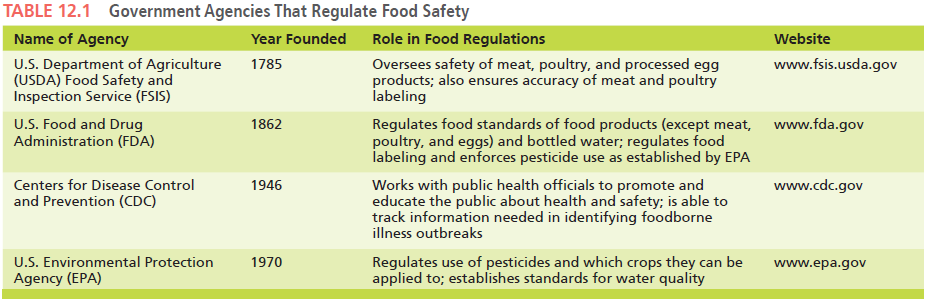
\includegraphics[width=\textwidth]{12_government_regulation_agencies}
	\caption{Government Regulation Agencies}
	\label{fig:government-regulation-agencies}
\end{figure}

\section{Food Production – Changes over 100 years}\label{sec:food-production--changes-over-100-years}
\begin{itemize}
	\item Has become increasingly complex
	\item Oversight has decreased
	\item More foods are mass-produced
	\item Ingredients come from various sources
	\item Contamination can occur at any point from farm to table
\end{itemize}

\begin{figure}[H]
	\centering
	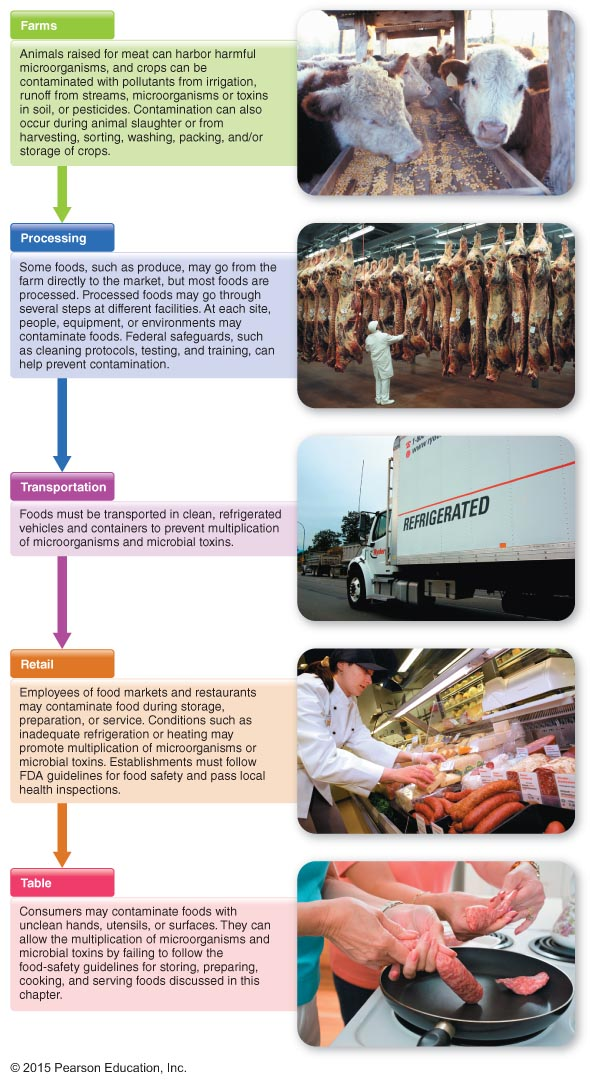
\includegraphics[height=0.7\paperheight]{12_food_from_farm_to_table}
	\caption{Food from Farm to Table}
	\label{fig:food-from-farm-to-table}
\end{figure}

\section{Causes of Foodborne Illness}\label{sec:causes-of-foodborne-illness}
\begin{itemize}
	\item Two types of foodborne illness
	\begin{itemize}
		\item \emph{Food infection}
		\begin{itemize}
			\item Illness resulting from eating food contaminated with living organisms
		\end{itemize}
	\end{itemize}
	\begin{itemize}
		\item \emph{Food intoxication}
		\begin{itemize}
			\item Illness resulting from eating food in which microbes have secreted toxins (poisons)
		\end{itemize}
	\end{itemize}
	\item Viruses and bacteria are the most common microbes causing foodborne illnesses
	\item Other sources of contamination include parasites, fungi, and prions
\end{itemize}

\subsection{Norovirus}\label{subsec:norovirus}

Of the viruses, norovirus causes more foodborne illness than the other 30 known pathogens put together\\
Often referred to as “the stomach flu”\\
Affects 19–21 million infections per year

\begin{figure}[H]
	\centering
	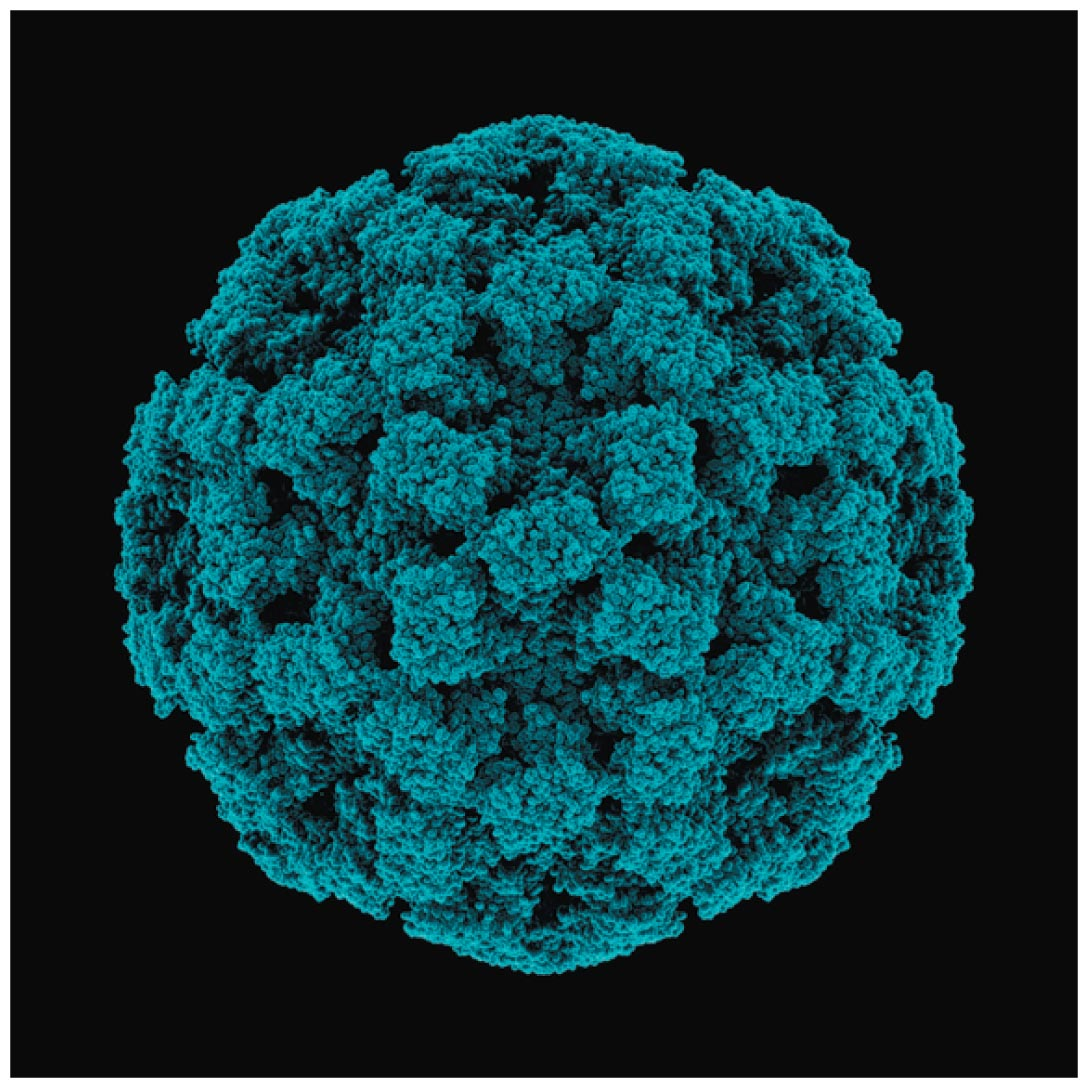
\includegraphics[width=0.5\textwidth]{12_norovirus}
	\caption{Norovirus}
	\label{fig:}
\end{figure}

%\vspace*{0.2\paperheight}
% FIXME: Add proper spacing under the wrap fig so nothing else is affected
\pagebreak

\begin{itemize}
	\item The most common bacterial causes of foodborne illness are
	\begin{itemize}
		\item Salmonella
		\item Clostridium perfringens
		\item Campylobacter
		\item Staphylococcus aureus
		\item Escherichia coli
		\item Listeria monocytogenes
	\end{itemize}
	\item The most deadly is \_\_\_\_\_\_\_\_\_\_\_\_\_
\end{itemize}

\begin{figure}[H]
	\centering
	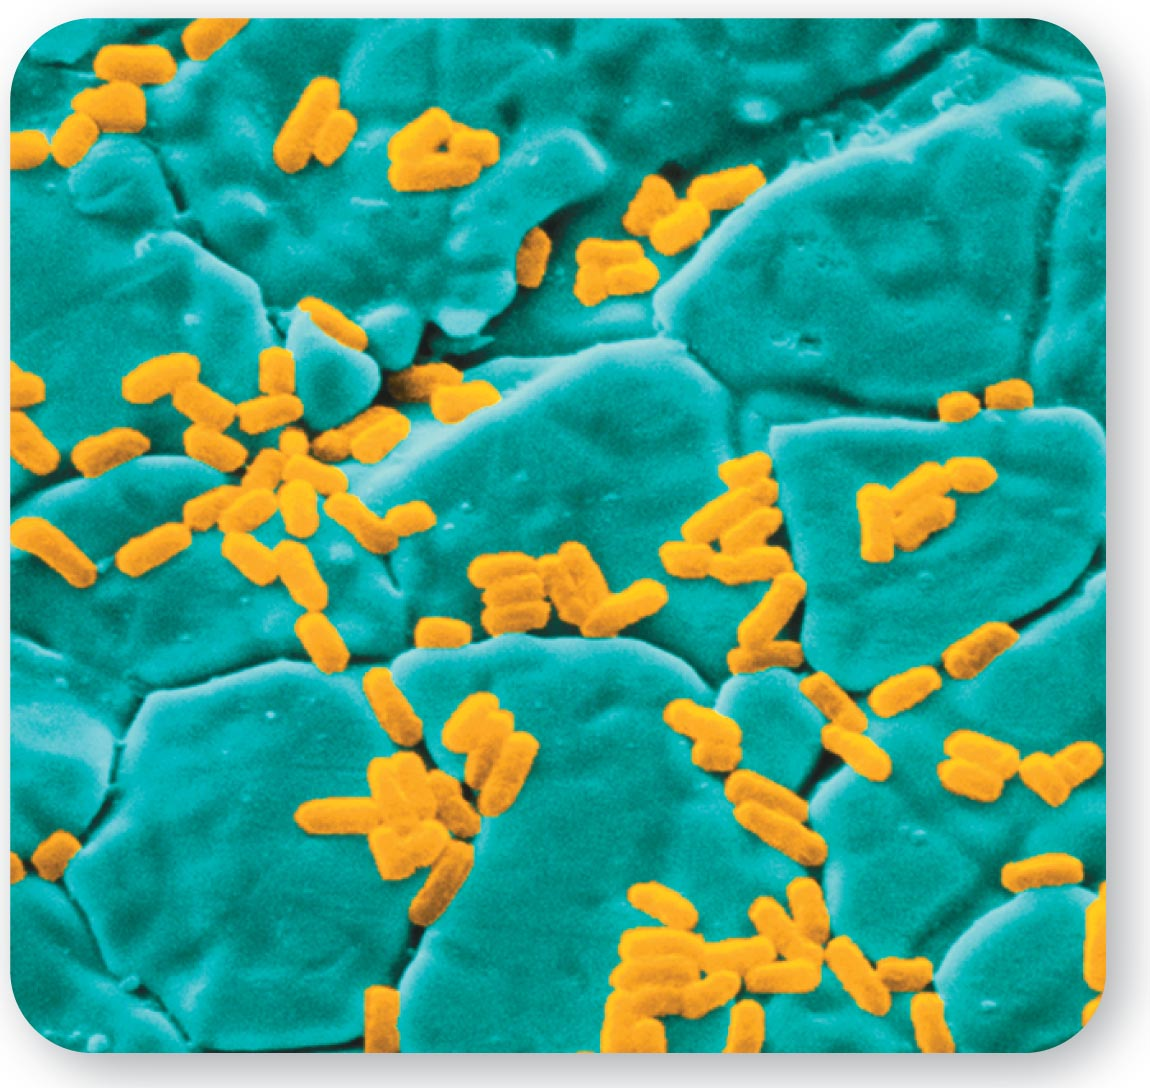
\includegraphics[width=\textwidth]{12_salmonella}
	\caption{Salmonella}
	\label{fig:salmonella}
\end{figure}

\begin{figure}[H]
	\centering
	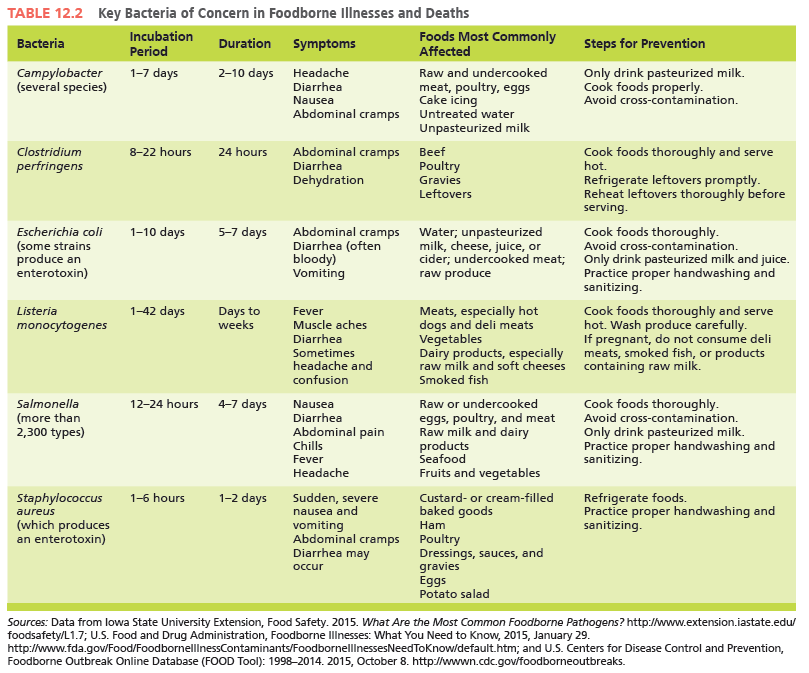
\includegraphics[width=\textwidth]{12_bacterial_causes_of_foodborne_illness}
	\caption{Bacterial Causes of Foodborne Illness}
	\label{fig:bacterial-causes-of-foodborne-illness}
\end{figure}

\begin{itemize}
	\item \definition{Parasites}{microorganisms that simultaneously derive benefit from and harm their host}
	\begin{itemize}
		\item Only responsible for about 2\% of foodborne illnesses
		\item Most common examples are helminths and protozoa
	\end{itemize}
	\item Other microorganisms causing illness include
	\begin{itemize}
		\item Viruses such as hepatitis A
		\item \emph{Helminths} or worms, such as tapeworms, flukes, and roundworms
		\item Giardia, causing a diarrheal illness called giardiasis
		\item \emph{Protozoa} are most commonly the cause of waterborne illness
		\item \emph{Fungi} (yeast and mold), which cause food spoilage
	\end{itemize}
\end{itemize}

\begin{figure}[H]
	\centering
	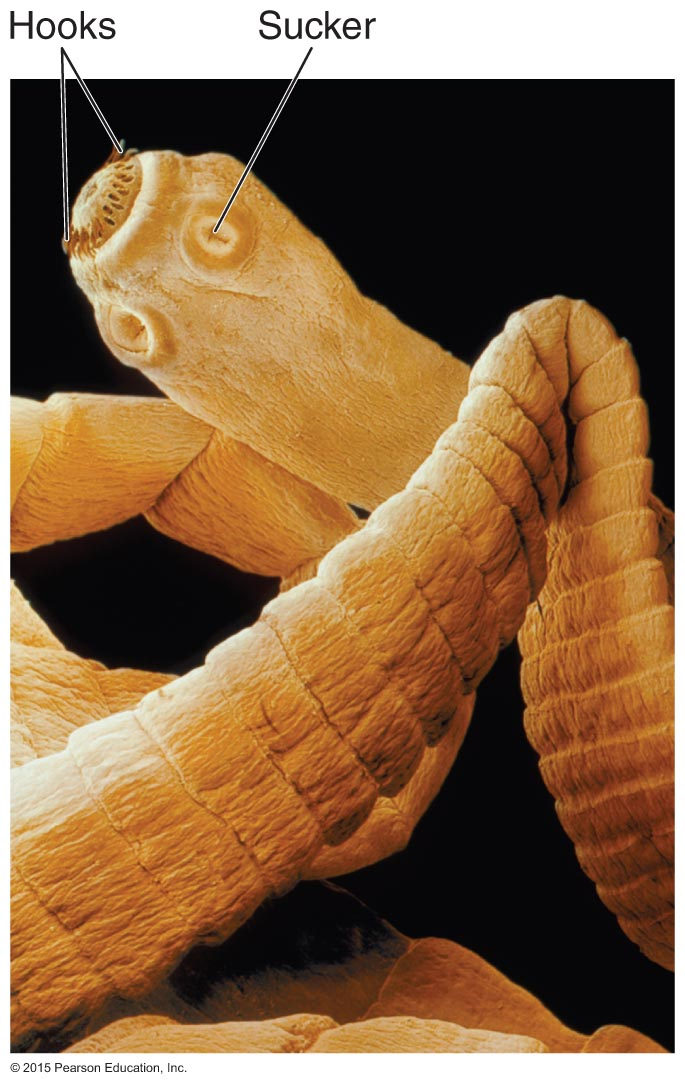
\includegraphics[height=0.7\textwidth]{12_tapeworms}
	\caption{Tapeworms}
	\label{fig:tapeworms}
\end{figure}

\begin{figure}[H]
	\centering
	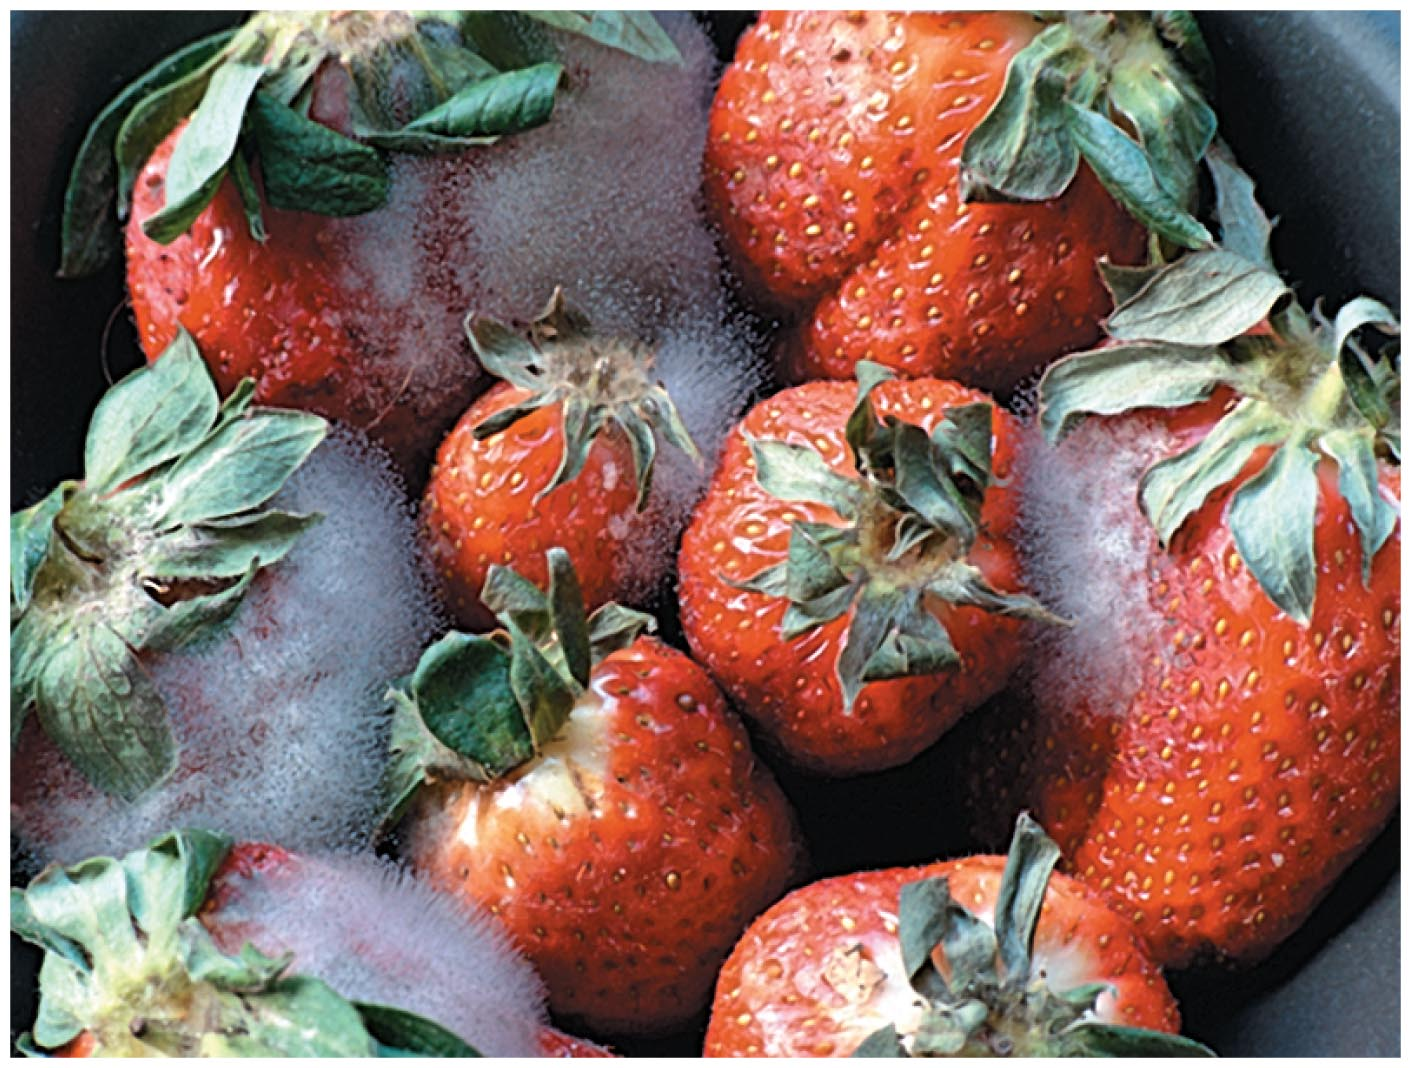
\includegraphics[width=\textwidth]{12_molds}
	\caption{Molds}
	\label{fig:molds}
\end{figure}

\begin{itemize}
	\item Some microbes cause illness by secreting toxins
	\begin{itemize}
		\item Clostridium botulinum produces \emph{botulism} toxin, which blocks nerve transmissions to muscle cells
		\item Toxins can be neurotoxins (damage the nervous system) or enterotoxins (damage the gastrointestinal tract)
		\item Fungi produce mycotoxins
		\item Toxic algae can contaminate fish and shellfish
		\item A variety of plant toxins can also cause illness
	\end{itemize}
\end{itemize}

\begin{figure}[H]
	\centering
	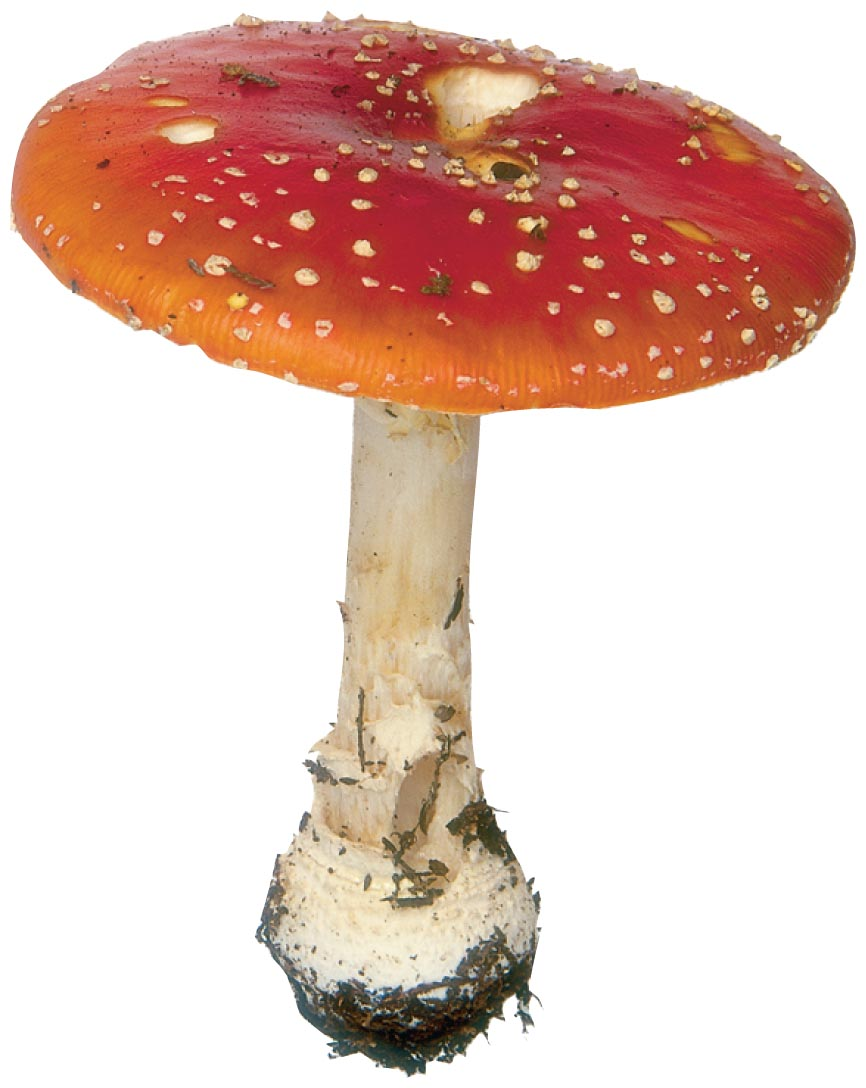
\includegraphics[width=\textwidth]{12_mushrooms_can_contain_dangerous_toxins}
	\caption{Mushrooms Can Contain Dangerous Toxins}
	\label{fig:mushrooms-can-contain-dangerous-toxins}
\end{figure}

\section{Conditions That Help Microbes Multiply}\label{sec:conditions-that-help-microbes-multiply}
\begin{itemize}
	\item Four factors affect the survival and reproduction of food microorganisms:
	\begin{enumerate}[label=\arabic*.,font=\bfseries\color{fdsnred}]
		\item Those that can cause human illness thrive in the temperature danger zone
		\item Many thrive in environments of high humidity
		\item Most have a preferred acidity range
		\item Many—though not all—depend on oxygen content to function
	\end{enumerate}
\end{itemize}

\begin{figure}[H]
	\centering
	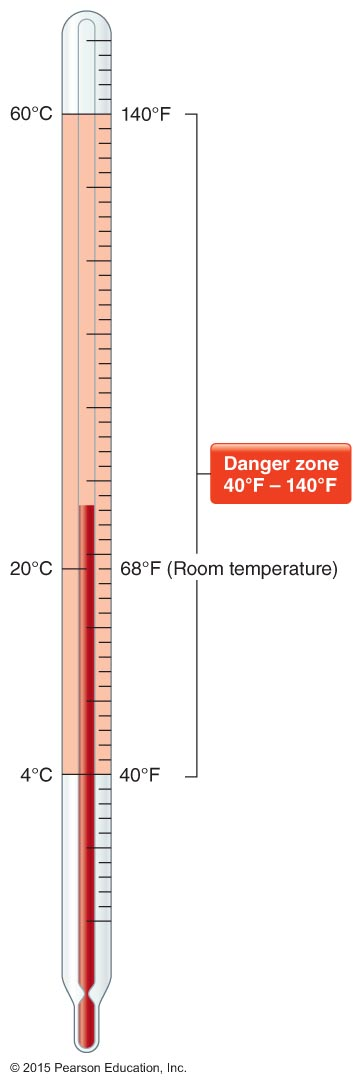
\includegraphics[height=0.5\paperwidth]{12_the_danger_zone}
	\caption{The Danger Zone}
	\label{fig:the-danger-zone}
\end{figure}

\section{Preventing Foodborne Illness}\label{sec:preventing-foodborne-illness}
When preparing foods at home, be sure to
\begin{itemize}
	\item Wash hands and kitchen surfaces often
	\item Separate foods to prevent \emph{cross-contamination}
	\item Chill or freeze foods to prevent microbes from growing
	\item Cook foods to their proper temperature
\end{itemize}

\begin{figure}[H]
	\centering
	
\includegraphics[width=\textwidth]{12_reducing_foodborne_illness}
	\caption{Reducing Foodborne Illness}
	\label{fig:reducing-foodborne-illness}
\end{figure}

\begin{figure}[H]
	\centering
	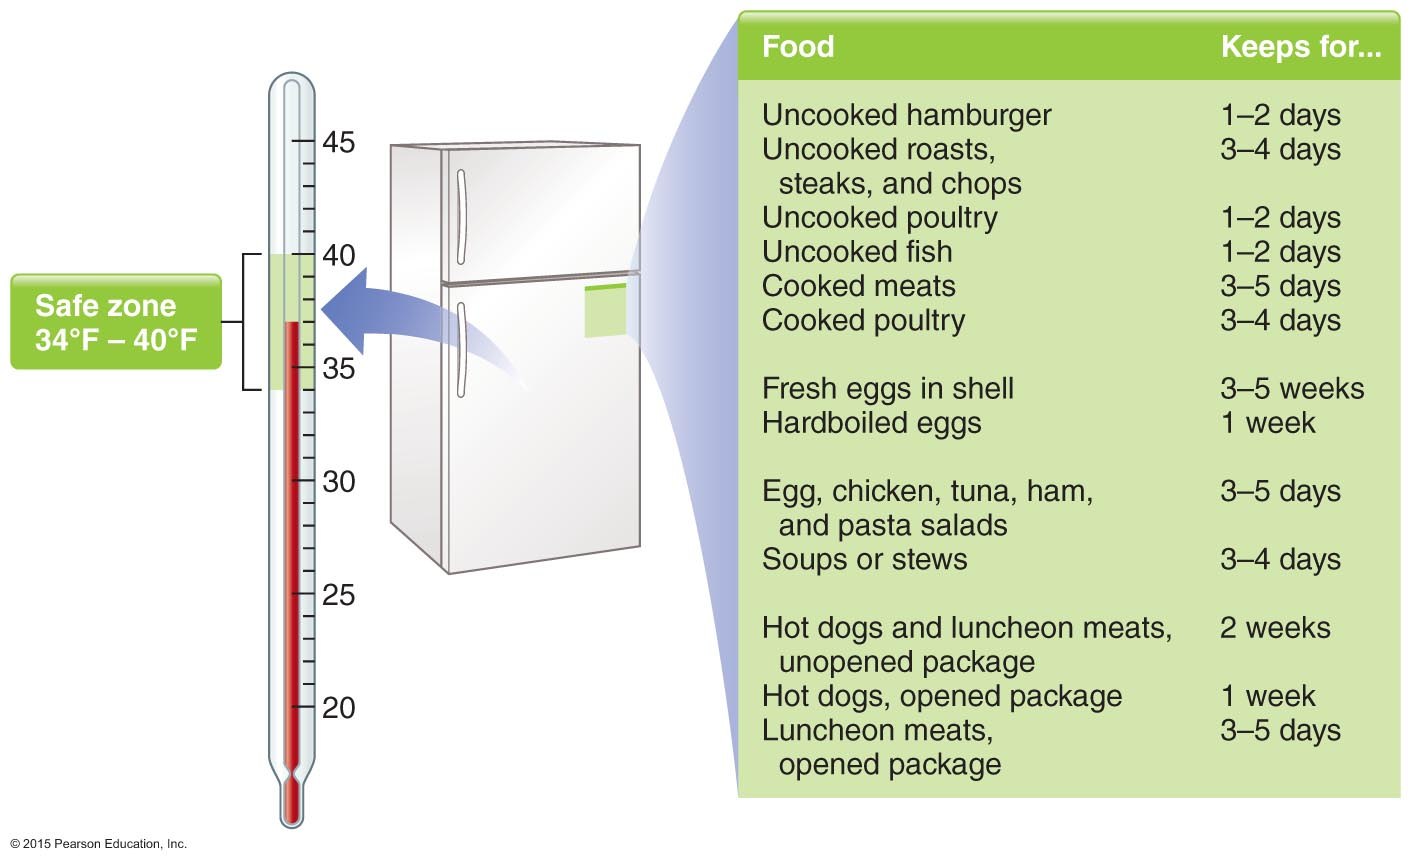
\includegraphics[width=\textwidth]{12_keeping_foods_refrigerated}
	\caption{Keeping Foods Refrigerated}
	\label{fig:keeping-foods-refrigerated}
\end{figure}

\begin{itemize}
	\item Foods should be cooked thoroughly to kill microbes
	\item Leftovers should be stored in the refrigerator for a limited period of time
	\item Food should be thawed slowly in the refrigerator
	\item When shopping, purchase refrigerated and frozen foods last
\end{itemize}

\begin{figure}[H]
	\centering
	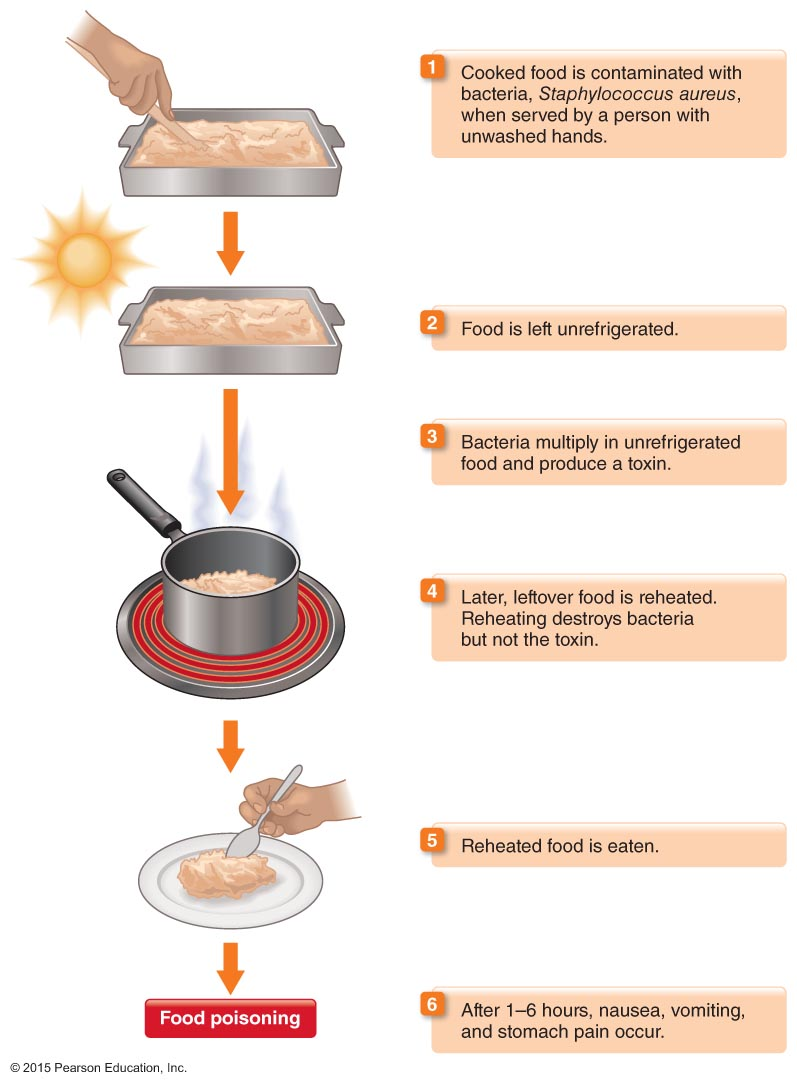
\includegraphics[width=\textwidth]{12_food_contamination}
	\caption{Food Contamination}
	\label{fig:food-contamination}
\end{figure}

\begin{itemize}
	\item When eating out:
	\begin{itemize}
		\item Eat at restaurants that look clean
		\item Insist that food be cooked thoroughly
	\end{itemize}
	\item When traveling:
	\begin{itemize}
		\item Avoid raw foods, salads, unpasteurized milk, and uncooked fruits and vegetables
		\item Select beverages carefully
		\item Use a waterless antibacterial hand cleanser frequently
	\end{itemize}
\end{itemize}

\section{Preventing Food Spoilage}\label{sec:preventing-food-spoilage}
\begin{itemize}
	\item Spoilage can be prevented by many natural techniques
	\begin{itemize}
		\item Salting or sugaring
		\item Drying
		\item Smoking
		\item Cooling
	\end{itemize}
	\item More modern techniques of preventing spoilage include
	\begin{itemize}
		\item Canning
		\item Pasteurization
		\item Irradiation
		\item Aseptic packaging
		\item Modified atmosphere packaging
		\item High-pressure processing
	\end{itemize}
\end{itemize}

\begin{figure}[H]
	\centering
	
\includegraphics[width=0.5\textwidth]{12_usda_radura}
	\caption{The USDA’s Radura}
	\label{fig:12-usda-radura}
\end{figure}

\section{Food Additives}\label{sec:food-additives}
\begin{itemize}
	\item Food additives are chemicals that do not occur naturally in the food but are added to enhance the food in some way – can include:
	\begin{itemize}
		\item Nutrients and preservatives
		\item Flavorings
		\item Colorings
		\item Other agents
	\end{itemize}
	\item More than 3,000 food additives are used in the United States
\end{itemize}

\begin{figure}[H]
	\centering
	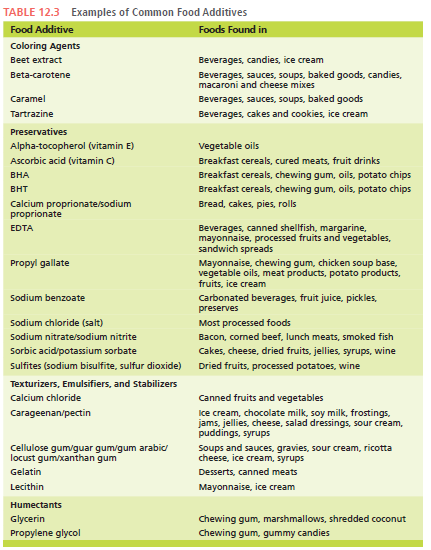
\includegraphics[width=\textwidth]{12_common_food_additives}
	\caption{Common Food Additives}
	\label{fig:common-food-additives}
\end{figure}

\begin{itemize}
	\item \emph{Sulfates} and \emph{nitrites} are preservatives that have raised health concerns
	\item Before a new additive can be used in food, the producer must demonstrate its safety to the FDA
	\item Substances already recognized as safe and exempt from stringent testing are referred to as \emph{generally recognized as safe (GRAS)}
\end{itemize}

\section{Genetic Modification in Food Production}\label{sec:genetic-modification-in-food-production}
\begin{itemize}
	\item In \emph{genetic modification}, the DNA of an organism is altered to bring about changes in its seeds or offspring
	\begin{itemize}
		\item \emph{Recombinant DNA technology} is a type of genetic modification in which DNA from different sources is combined
		\item An increasing number and quantity of food crops have been genetically modified
	\end{itemize}
\end{itemize}

\begin{figure}[H]
	\centering
	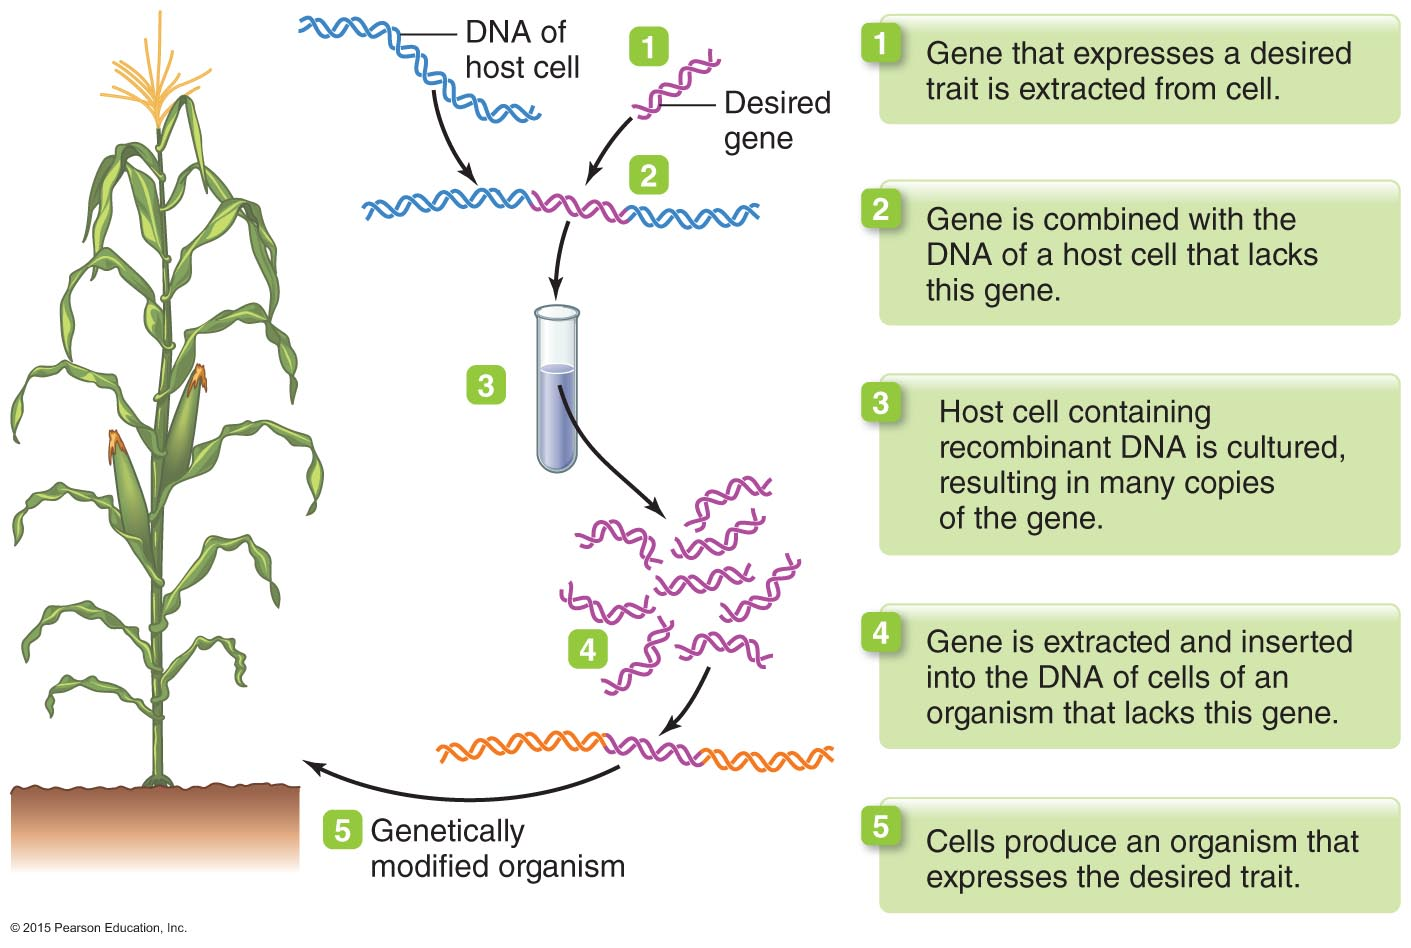
\includegraphics[width=\textwidth]{12_recombinant_dna_technology}
	\caption{Recombinant DNA Technology}
	\label{fig:recombinant-dna-technology}
\end{figure}

\section{Benefits to Genetic Modification}\label{sec:benefits-to-genetic-modification}
\begin{itemize}
	\item GM crops grow faster and have a higher yield
	\item Drought-resistant crops help to conserve water
	\item Reduced energy use to grow, pesticides, emissions from greenhouse gases, and increased soil preservation
	\item GM crops can be produced with higher nutrient contents
	\item Improved farmer profits benefit the economy
	\item Health risks
	\begin{itemize}
		\item \definition{Allergenicity}{genes transferred from common allergen foods could affect those with allergies}
		\begin{itemize}
			\item No currently reports however
		\end{itemize}
		\item Consuming crops that are antimicrobial could potential hard the cells of our body or our microbial flora in the GI tract
		\item Genes from GM crops have migrated to conventional crops miles away
		\item Possible link to cancer
	\end{itemize}
	\item Environmental risks
	\begin{itemize}
		\item Loss of biodiversity
		\item Generation of superweeds
		\item Threats to other species
	\end{itemize}
	\item Economic instability
\end{itemize}

\section{Should We Label GM Foods?}\label{sec:should-we-label-gm-foods?}
\begin{itemize}
	\item Labeling would allow consumers to know if their food contained GM products
	\item The European Union has long required that GM foods are labeled clearly
	\item In 2016 the FDA did not require such labeling
	\item GM crops have been used in the United States for 20 years without labeling
\end{itemize}

\section{Residues on Foods}\label{sec:residues-on-foods}
\begin{itemize}
	\item Various chemicals can persist and even accumulate in foods
	\item These residues can include
	\begin{itemize}
		\item Persistent organic pollutants
		\item Insecticides, herbicides, and fungicides
		\item Growth hormone
	\end{itemize}
\end{itemize}

\section{Persistent Organic Pollutants}\label{sec:persistent-organic-pollutants}
\begin{itemize}
	\item Persistent organic pollutants (POPs): chemicals released into the atmosphere from industry, agriculture, automobiles, and waste disposal
	\begin{itemize}
		\item Found in virtually all categories of foods
		\item Include
		\begin{itemize}
			\item Mercury and lead, which are nerve toxins
			\item Dioxins, which increase risk of cancer and other disorders
		\end{itemize}
	\end{itemize}
\end{itemize}

\begin{figure}[H]
	\centering
	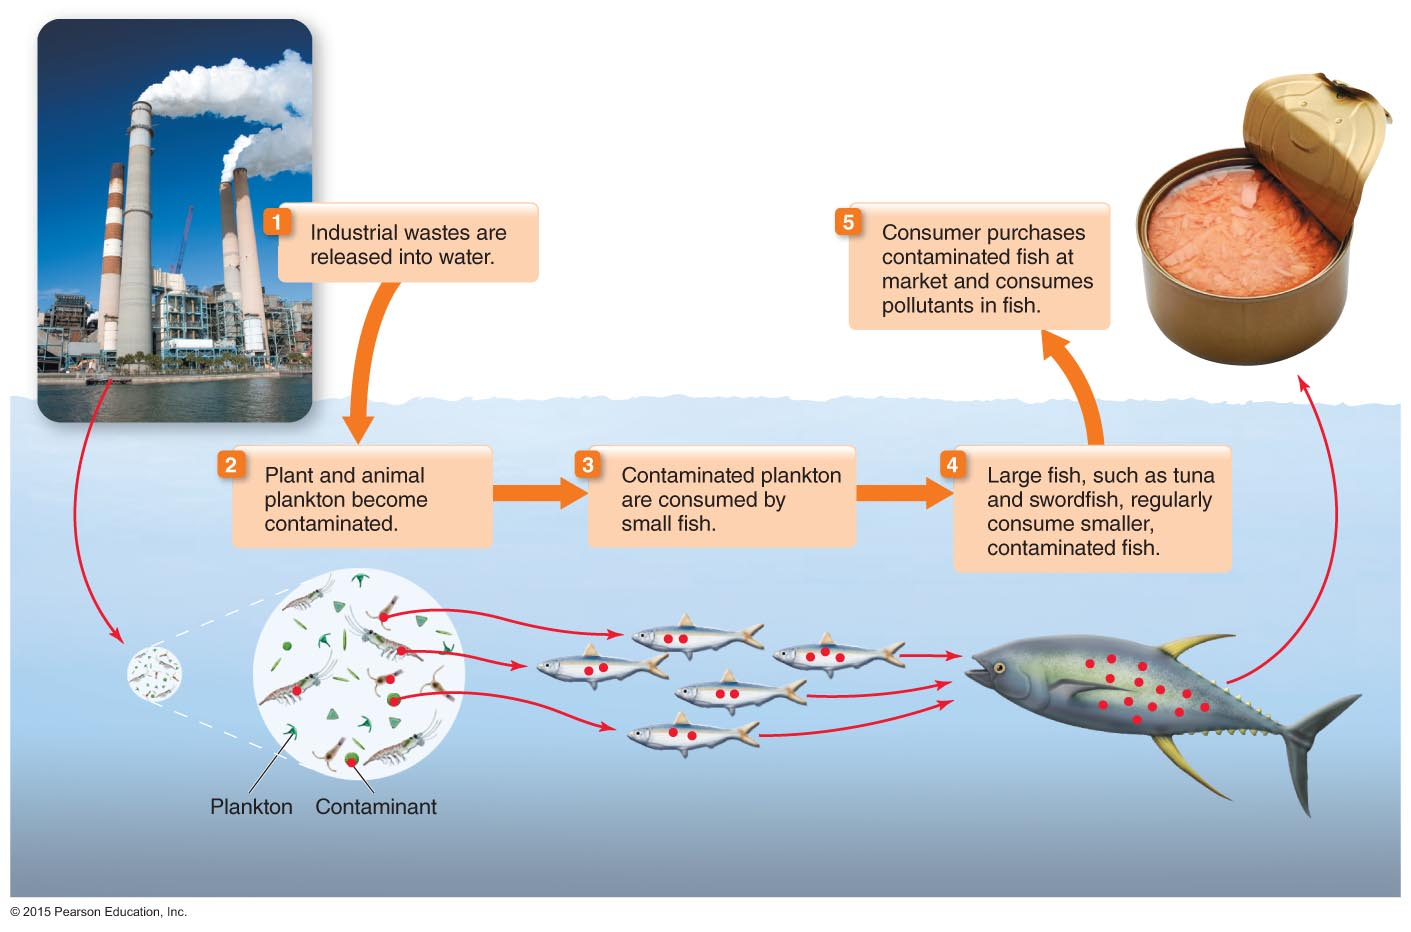
\includegraphics[width=\textwidth]{12_biomagnification_of_pops}
	\caption{Biomagnification of POPs}
	\label{fig:biomagnification-of-pops}
\end{figure}

\section{Pesticides}\label{sec:pesticides}
\begin{itemize}
	\item Pesticides are used to help protect against crop losses, reduce the incidence of disease, and increase crop yields
	\begin{itemize}
		\item Most common are insecticides, herbicides, and fungicides
		\item Can be natural or synthetic
		\item Can remain as toxins on foods
		\item Regulated by the EPA
	\end{itemize}
\end{itemize}

\section{Growth Hormones and Antibiotics}\label{sec:growth-hormones-and-antibiotics}
\begin{itemize}
	\item \emph{Recombinant bovine growth hormone (rBGH)} is a genetically engineered growth hormone given to cows
	\begin{itemize}
		\item Increases muscle mass; decreases fat
		\item Increases milk production
		\item One-third of all U.S.\ dairy cows receive rBGH
		\item Risks to humans are still being studied
	\end{itemize}
	\item Antibiotics are routinely given to animals raised for food to reduce the number of disease outbreaks
	\begin{itemize}
		\item Risks to humans are still being studied
		\item May be developing significant reservoirs for antibiotic-resistant strains of bacteria, or ``superbugs''
	\end{itemize}
	\item Exposure to growth hormones and antibiotics can be reduced by selecting organic foods, free-range meats, and vegetarian meals
\end{itemize}

\section{Organic Foods}\label{sec:organic-foods}
\begin{itemize}
	\item Organic foods are grown without the use of synthetic pesticides
	\begin{itemize}
		\item Standards for organic production are regulated by the USDA
	\end{itemize}
	\begin{description}
		\item[100\% organic:] only organic ingredients
		\item[Organic:] 95\% of ingredients are organic
		\item[Made with organic ingredients:] 70\% or more of ingredients are organic
	\end{description}
\end{itemize}

\begin{figure}[H]
	\centering
	
\includegraphics[width=0.5\textwidth]{12_usda_organic_seal}
	\caption{USDA Organic Seal}
	\label{fig:usda-organic-seal}
\end{figure}

\section{In Depth: Supplements}\label{sec:in-depth:-supplements}
\begin{itemize}
	\item \emph{Supplements}, according to the FDA, are a product containing ingredients like vitamins, minerals, herms, amino acids, or enzymes
	\item In 2014 sales of dietary supplements reached nearly \$37 billion
	\item Are supplements safe?
	\begin{itemize}
		\item In 2015, 14 U.S.\ Attorneys General signed a letter to congress requesting for an investigation of the dietary supplement industry
		\item This comes after an audit for DNA testing of ingredients found they did not contain ingredients listed, but did contain heavy metals
	\end{itemize}
\end{itemize}

\begin{figure}[H]
	\centering
	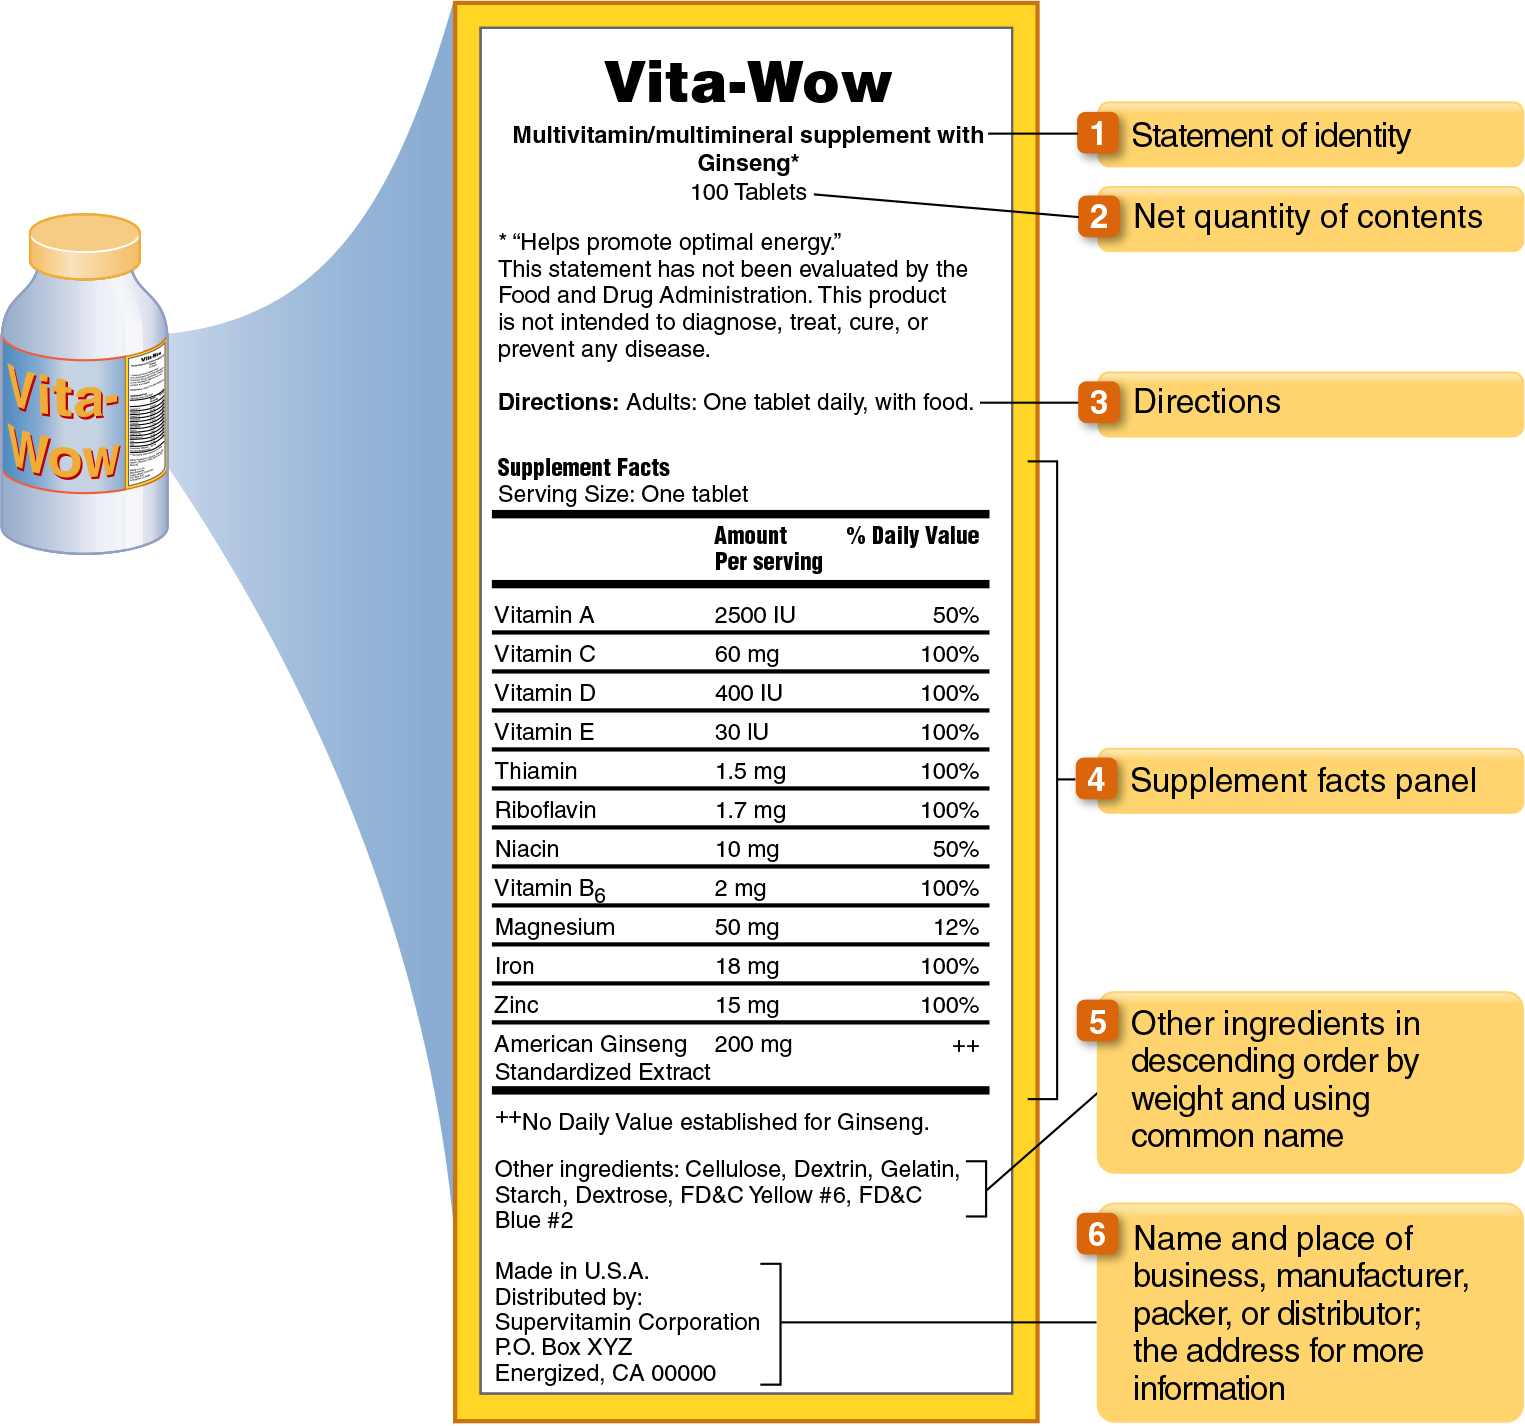
\includegraphics[width=\textwidth]{12_supplements}
	\caption{Supplements}
	\label{fig:supplements}
\end{figure}

\begin{itemize}
	\item The FDA does not have the authority to review safety and efficacy of supplements
	\item It is the responsibility of the manufacturer to prove the safety of supplements
	\item Manufacturers do not have to tell the FDA they have added an ingredient
	\item The FDA does not regulate practices to ensure the purity
\end{itemize}

\subsection{Herbal supplements}\label{subsec:herbal-supplements}
\begin{itemize}
	\item The plant or part of the plant that is used to flavor, scent, and/or potential health-related properties
	\item The National Center for Complimentary and Integrative Health (NCCIH)
	\item Consult a healthcare provider before beginning a supplement
\end{itemize}

\begin{figure}[H]
	\centering
	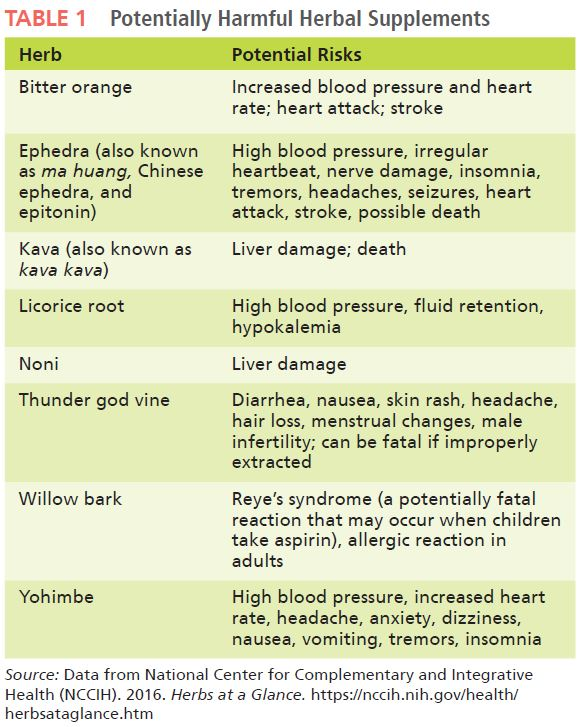
\includegraphics[width=\textwidth]{12_potentially_harmful_herbal_supplements}
	\caption{Potentially Harmful Herbal Supplements}
	\label{fig:12-potentially-armful-erbal-supplements}
\end{figure}

\begin{itemize}
	\item Surveys show that 67\% of Americans use a vitamin or mineral supplement
	\begin{itemize}
		\item 35\% use “specialty” supplements
		\item 23\% use botanicals
		\item 17\% use sports supplements
	\end{itemize}
\end{itemize}

\begin{figure}[H]
	\centering
	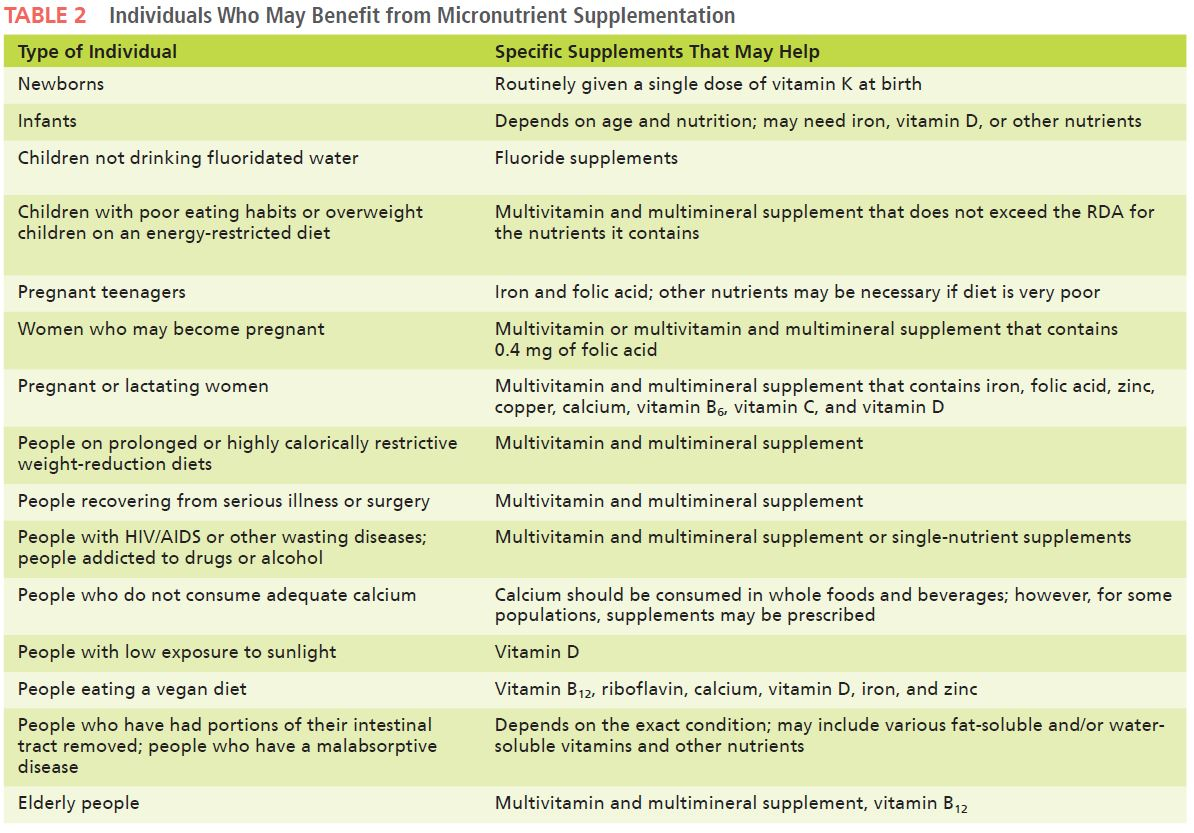
\includegraphics[width=\textwidth]{12_image21}
	\caption{Individuals Who May Benefit from Micronutrient Supplementation}
	\label{fig:micronutrient-supplementation}
\end{figure}

%</Chapter12>

\end{document}
